%% LyX 2.3.4.2 created this file.  For more info, see http://www.lyx.org/.
%% Do not edit unless you really know what you are doing.
\documentclass[english,dvipsnames,aspectratio=169]{beamer}
\usepackage{mathptmx}
\usepackage{eulervm}
\usepackage[T1]{fontenc}
\usepackage[latin9]{inputenc}
\usepackage{babel}
\usepackage{amstext}
\usepackage{amssymb}
\usepackage{graphicx}
\usepackage{ifthen}
\usepackage{xcolor}
\usepackage{xspace}
\usepackage{tikz}
\usetikzlibrary{tikzmark}
\usetikzlibrary{calc}
\usepackage{pgfplots}
%\pgfplotsset{compat=1.17}
\usepackage{booktabs}
\usepackage{xpatch}

\xpatchcmd{\itemize}
  {\def\makelabel}
  {\ifnum\@itemdepth=1\relax
     \setlength\itemsep{2ex}% separation for first level
   \else
     \ifnum\@itemdepth=2\relax
       \setlength\itemsep{1ex}% separation for second level
     \else
       \ifnum\@itemdepth=3\relax
         \setlength\itemsep{0.5ex}% separation for third level
   \fi\fi\fi\def\makelabel
  }
 {}
 {}

\ifx\hypersetup\undefined
  \AtBeginDocument{%
    \hypersetup{unicode=true,pdfusetitle,
 bookmarks=true,bookmarksnumbered=false,bookmarksopen=false,
 breaklinks=false,pdfborder={0 0 0},pdfborderstyle={},backref=false,colorlinks=true,
 allcolors=NYUPurple,urlcolor=LightPurple}
  }
\else
  \hypersetup{unicode=true,pdfusetitle,
 bookmarks=true,bookmarksnumbered=false,bookmarksopen=false,
 breaklinks=false,pdfborder={0 0 0},pdfborderstyle={},backref=false,colorlinks=true,
 allcolors=NYUPurple,urlcolor=LightPurple}
\fi

\makeatletter

%%%%%%%%%%%%%%%%%%%%%%%%%%%%%% LyX specific LaTeX commands.
%% Because html converters don't know tabularnewline
\providecommand{\tabularnewline}{\\}

%%%%%%%%%%%%%%%%%%%%%%%%%%%%%% Textclass specific LaTeX commands.
% this default might be overridden by plain title style
\newcommand\makebeamertitle{\frame{\maketitle}}%
% (ERT) argument for the TOC
\AtBeginDocument{%
  \let\origtableofcontents=\tableofcontents
  \def\tableofcontents{\@ifnextchar[{\origtableofcontents}{\gobbletableofcontents}}
  \def\gobbletableofcontents#1{\origtableofcontents}
}

%%%%%%%%%%%%%%%%%%%%%%%%%%%%%% User specified LaTeX commands.
\usetheme{CambridgeUS} 
\beamertemplatenavigationsymbolsempty


% Set Color ==============================
\definecolor{NYUPurple}{RGB}{87,6,140}
\definecolor{LightPurple}{RGB}{165,11,255}


\setbeamercolor{title}{fg=NYUPurple}
\setbeamercolor{frametitle}{fg=NYUPurple}

\setbeamercolor{background canvas}{fg=NYUPurple, bg=white}
\setbeamercolor{background}{fg=black, bg=NYUPurple}

\setbeamercolor{palette primary}{fg=black, bg=gray!30!white}
\setbeamercolor{palette secondary}{fg=black, bg=gray!20!white}
\setbeamercolor{palette tertiary}{fg=gray!20!white, bg=NYUPurple}

\setbeamertemplate{headline}{}
\setbeamerfont{itemize/enumerate body}{}
\setbeamerfont{itemize/enumerate subbody}{size=\normalsize}

\setbeamercolor{parttitle}{fg=NYUPurple}
\setbeamercolor{sectiontitle}{fg=NYUPurple}
\setbeamercolor{sectionname}{fg=NYUPurple}
\setbeamercolor{section page}{fg=NYUPurple}
%\setbeamercolor{description item}{fg=NYUPurple}
%\setbeamercolor{block title}{fg=NYUPurple}

\setbeamertemplate{blocks}[rounded][shadow=false]
\setbeamercolor{block body}{bg=normal text.bg!90!NYUPurple}
\setbeamercolor{block title}{bg=NYUPurple!30, fg=NYUPurple}



\AtBeginSection[]{
  \begin{frame}
  \vfill
  \centering
\setbeamercolor{section title}{fg=NYUPurple}
 \begin{beamercolorbox}[sep=8pt,center,shadow=true,rounded=true]{title}
    \usebeamerfont{title}\usebeamercolor[fg]{title}\insertsectionhead\par%
  \end{beamercolorbox}
  \vfill
  \end{frame}
}

\makeatother

\setlength{\parskip}{\medskipamount} 

\input ../macros

\begin{document}
\input ../rosenberg-macros

\title[DS-GA 1003]{Regularization}
\author{He He\\\vspace{2em}{
    Slides based on Lecture
    \href{https://davidrosenberg.github.io/mlcourse/Archive/2019/Lectures/02c.L1L2-regularization.pdf}{2c}
    from David Rosenberg's \href{https://github.com/davidrosenberg/mlcourse}{course material}.
}}

\date{Feb 16, 2021}
\institute{CDS, NYU}

\makebeamertitle
\mode<article>{Just in article version}

\section{$\ell_2$ and $\ell_1$ Regularization}

\begin{frame}
    {Complexity Penalty}
    \head{Goal}: balance between complexity of the hypothesis space $\sF$ and the training loss

    \head{Complexity measure}: $\Omega:\cf\to[0,\infty)$, e.g. number of features

\begin{block}{Penalized ERM (Tikhonov regularization)}

For complexity measure $\Omega:\cf\to[0,\infty)$ and fixed $\lambda\ge0$,
\begin{align*}
\min_{f\in\cf} & \frac{1}{n}\sum_{i=1}^{n}\ell(f(x_{i}),y_{i})+\lambda\Omega(f)
\end{align*}
\end{block}

As usual, find $\lambda$ using validation data.

Number of features as complexity measure is hard to optimize---other measures?
\end{frame}

\begin{frame}
    {Weight Shrinkage: Intuition}
    Consider linear regression on the following data, which line would you prefer? [draw]
    \vspace{10em}
    \pause
    \begin{itemize}
        \item Prefer the line with \hl{smaller slope}: small change in the input does not cause large change in the output
        \item If the estimated weights change by a small amount, it wouldn't cause huge change in the prediction (\hl{less sensitive to data})
    \end{itemize}
\end{frame}

\begin{frame}
    {Weight Shrinkage: Polynomial Regression}
    \begin{figure}
        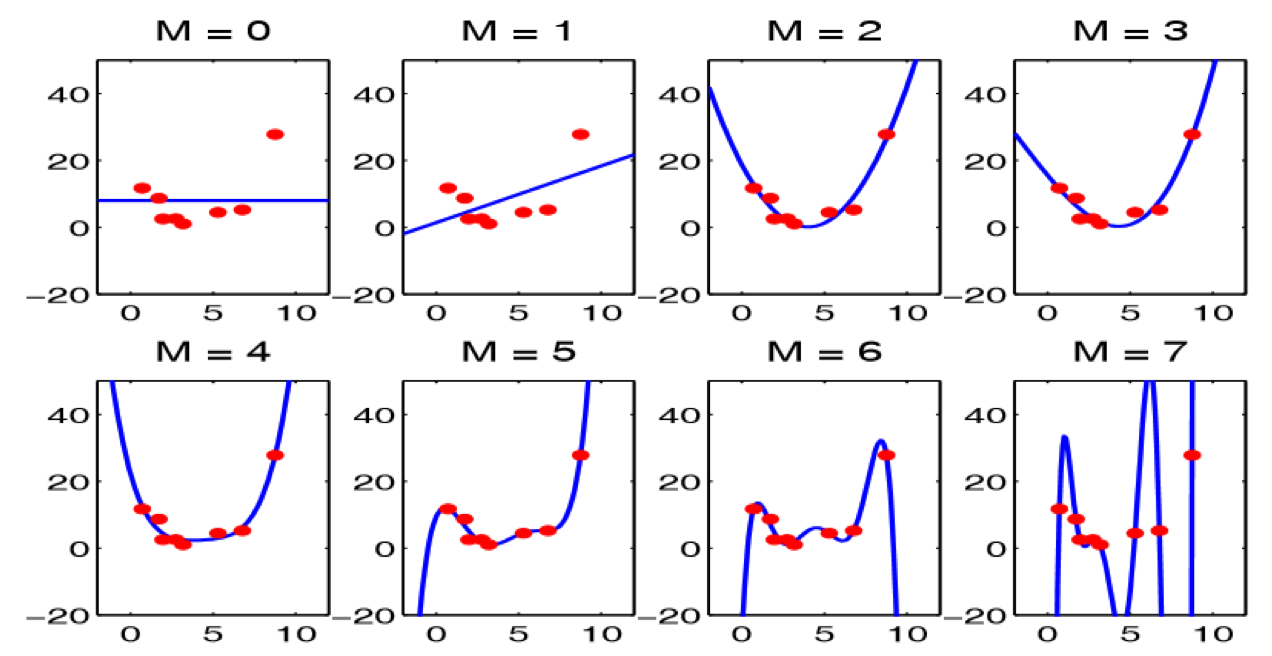
\includegraphics[height=4.5cm]{figures/poly-regression}
    \end{figure}
    \begin{itemize}
    \item Large weights are needed to ``wiggle'' the curve
    \item Want to regularize the weights to make them smaller, e.g.
        \begin{itemize}
            \item[] $\hat{y} = 0.001x^7 + 0.003x^3 + 1$ vs
                    $\hat{y} = 1000x^7 + 500x^3 + 1$
        \end{itemize}
    \end{itemize}
    \small{(Adapated from Mark Schmidt's slide)}
\end{frame}

\begin{frame}
    {Linear Regression with L2 Regularization}
\begin{itemize}
\item Consider linear models
\[
\cf=\left\{ f:\reals^{d}\to\reals\mid f(x)=w^{T}x\mbox{ for }w\in\reals^{d}\right\} 
\]
\item Square loss: $\loss(\hat{y},y)=\left(y-\hat{y}\right)^{2}$
\item Training data $\cd_{n}=\left((x_{1},y_{1}),\ldots,(x_{n},y_{n})\right)$
\item Linear least squares regression is ERM for square loss over $\cf$:
\[
\hat{w}=\argmin_{w\in\reals^{d}}\frac{1}{n}\sum_{i=1}^{n}\left\{ w^{T}x_{i}-y_{i}\right\} ^{2}
\]
\item Can overfit when $d$ is large compared to $n$, 
e.g. $d\gg n$ very common in NLP 
(e.g. a 1M features for 10K documents).
\end{itemize}
\end{frame}

\begin{frame}
    {Linear Regression with L2 Regularization}
    \hl{Penalize ``large'' weights} where size of weights is measured by $\ell_2$ norm:
\[
\hat{w}=\argmin_{w\in\reals^{d}}\frac{1}{n}\sum_{i=1}^{n}\left\{ w^{T}x_{i}-y_{i}\right\} ^{2}+
    {\color{blue}\lambda\|w\|_{2}^{2}},
\]
where $\|w\|_{2}^{2}=w_{1}^{2}+\cdots+w_{d}^{2}$ is the square of
the $\ell_{2}$-norm.

\medskip
\begin{itemize}
    \item Also known as \textbf{ridge regression}.
    \item We get back linear least square regression with $\lambda=0$.
    \item $\ell_2$ regularization can be used for other models too (e.g. neural networks)
\end{itemize}
\end{frame}

\begin{frame}{How does $\ell_{2}$ regularization induce ``regularity''?}
\begin{itemize}
    \item Short answer: it controls ``sensitivity'' of the function.
\item For $\hat{f}(x)=\hat{w}^{T}x$, $\hat{f}$ is \textbf{Lipschitz continuous
}with Lipschitz constant $L=\|\hat{w}\|_{2}$.

\item That is, when moving from $x$ to $x+h$, $\hat{f}$ changes
no more than $L\|h\|$. 

\item So $\ell_{2}$ regularization controls the maximum rate of change
of $\hat{f}$.

\item Proof:
\begin{eqnarray*}
\left|\hat{f}(x+h)-\hat{f}(x)\right| & = & |\hat{w}^{T}\left(x+h\right)-\hat{w}^{T}x|=\left|\hat{w}^{T}h\right|\\
 & \le & \|\hat{w}\|_{2}\|h\|_{2}\quad\text{(Cauchy-Schwarz inequality)}
\end{eqnarray*}


\item Note that other norms also provides a bound on $L$ due to the equivalence of norms: $\exists C>0 \text{ s.t. } \|\hat{w}_2\|_2 \le C\|\hat{w}_2\|_p$
\end{itemize}
\end{frame}

\begin{frame}
    {Linear Regression vs Ridge Regression}
    \head{Objective}:\\
    \begin{itemize}
        \setlength\itemsep{1ex}
        \item Linear: $L(w) = \frac{1}{2}\|Xw - y\|_2^2$
        \item Ridge: $L(w) = \frac{1}{2}\|Xw - y\|_2^2 + {\color{blue}\frac{\lambda}{2}{\|w\|_2^2}}$
    \end{itemize}

    \head{Gradient}:\\
    \begin{itemize}
        \setlength\itemsep{1ex}
        \item Linear: $\nabla L(w) = X^T(Xw - y)$
        \item Ridge: $\nabla L(w) = X^T(Xw - y) + {\color{blue}\lambda w}$
            \begin{itemize}
                \item Also known as \textbf{weight decay} in neural networks
            \end{itemize}
    \end{itemize}

    \head{Closed-form solution}:\\
    \begin{itemize}
        \setlength\itemsep{1ex}
        \item Linear: $X^TXw = X^Ty$
        \item Ridge: $(X^TX + {\color{blue}\lambda I})w = X^Ty$
            \begin{itemize}
                \item $(X^TX + {\color{blue}\lambda I})$ is always invertible
            \end{itemize}
    \end{itemize}
\end{frame}

\begin{frame}{Ridge Regression: Regularization Path}
    \textbf{Regulariztion path} shows how the weights vary as we change the regularization strength

\let\thefootnote\relax\footnotetext{\tiny{Modified from Hastie, Tibshirani, and Wainwright's \emph{Statistical Learning with Sparsity}, Fig 2.1. About predicting crime in 50 US cities.}}
\begin{center}
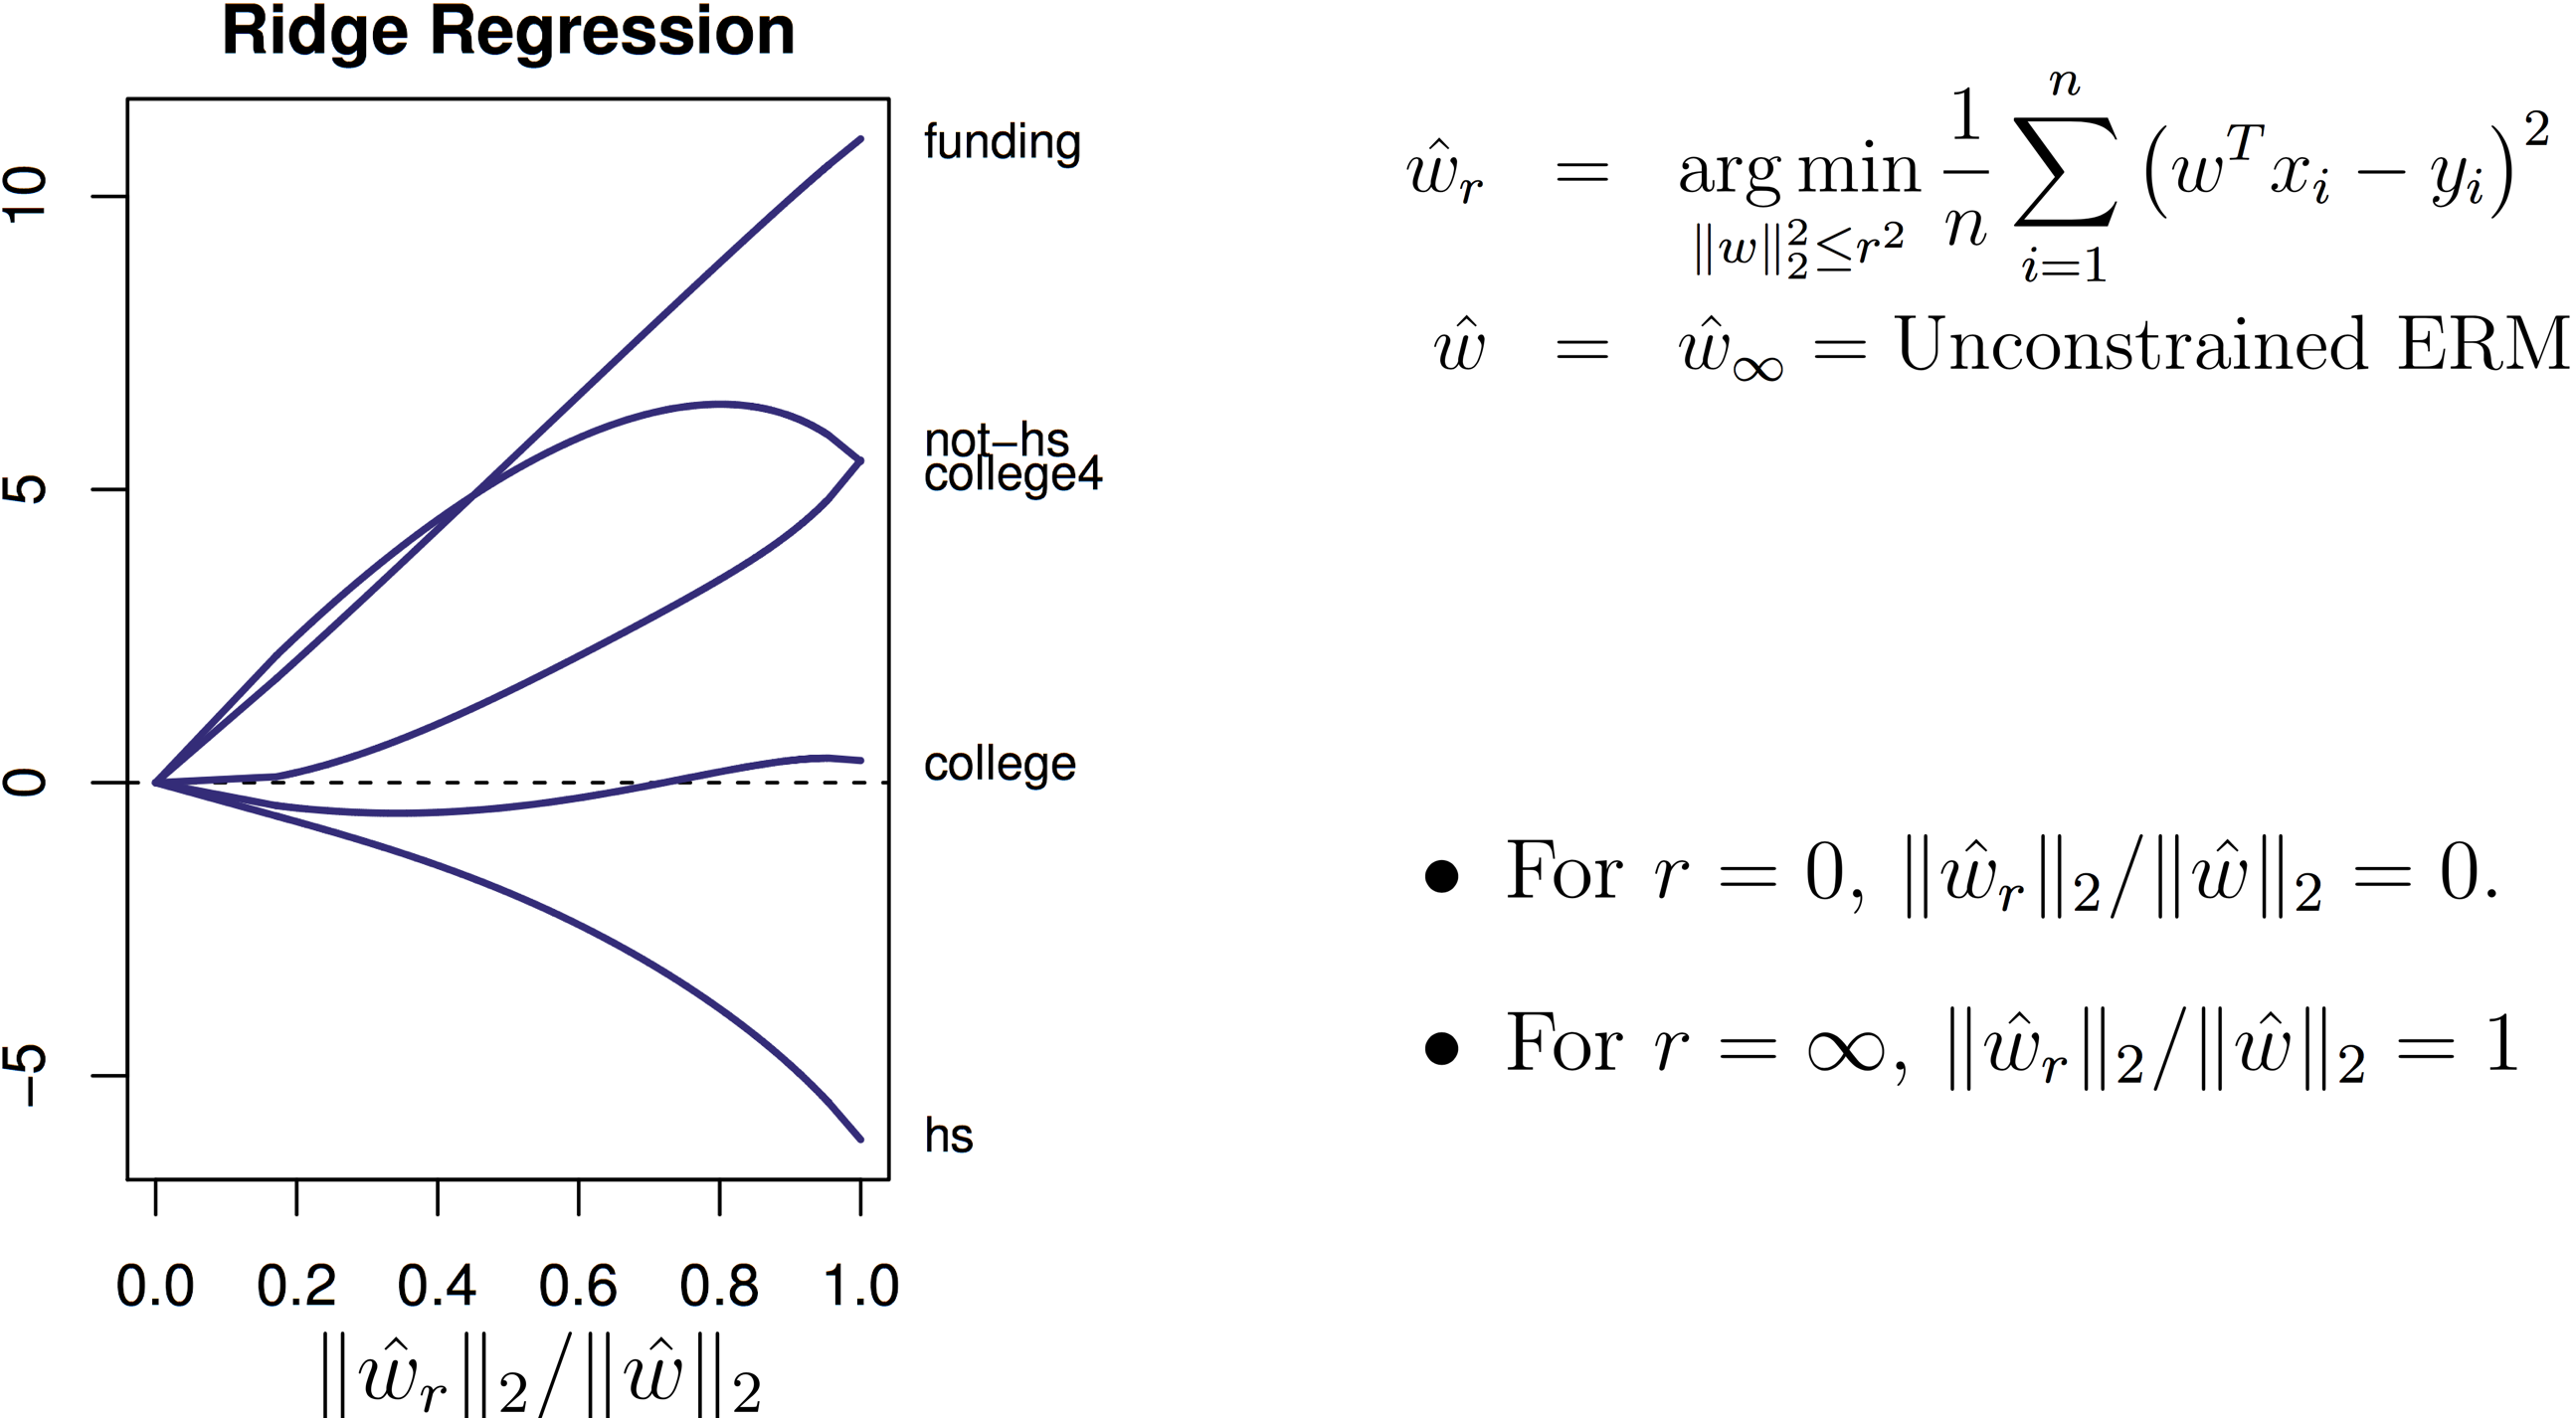
\includegraphics[height=0.7\textheight]{figures/ridge-regularization-HTW-Fig2.1-LATEX.png} 
\par\end{center}
\end{frame}

\begin{frame}{Lasso Regression}
    Penalize the $\ell_1$ norm of the weights:
\begin{block}{Lasso Regression (Tikhonov Form)}
\[
\hat{w}=\argmin_{w\in\reals^{d}}\frac{1}{n}\sum_{i=1}^{n}\left\{ w^{T}x_{i}-y_{i}\right\} ^{2}+\lambda\|w\|_{1},
\]
where $\|w\|_{1}=\left|w_{1}\right|+\cdots+\left|w_{d}\right|$ is
the $\ell_{1}$-norm.
\end{block}
\end{frame}

\begin{frame}{Ridge vs. Lasso: Regularization Paths}
Lasso gives sparse weights:

\let\thefootnote\relax\footnotetext{\tiny{Modified from Hastie, Tibshirani, and Wainwright's \emph{Statistical Learning with Sparsity}, Fig 2.1. About predicting crime in 50 US cities.}}
\begin{center}
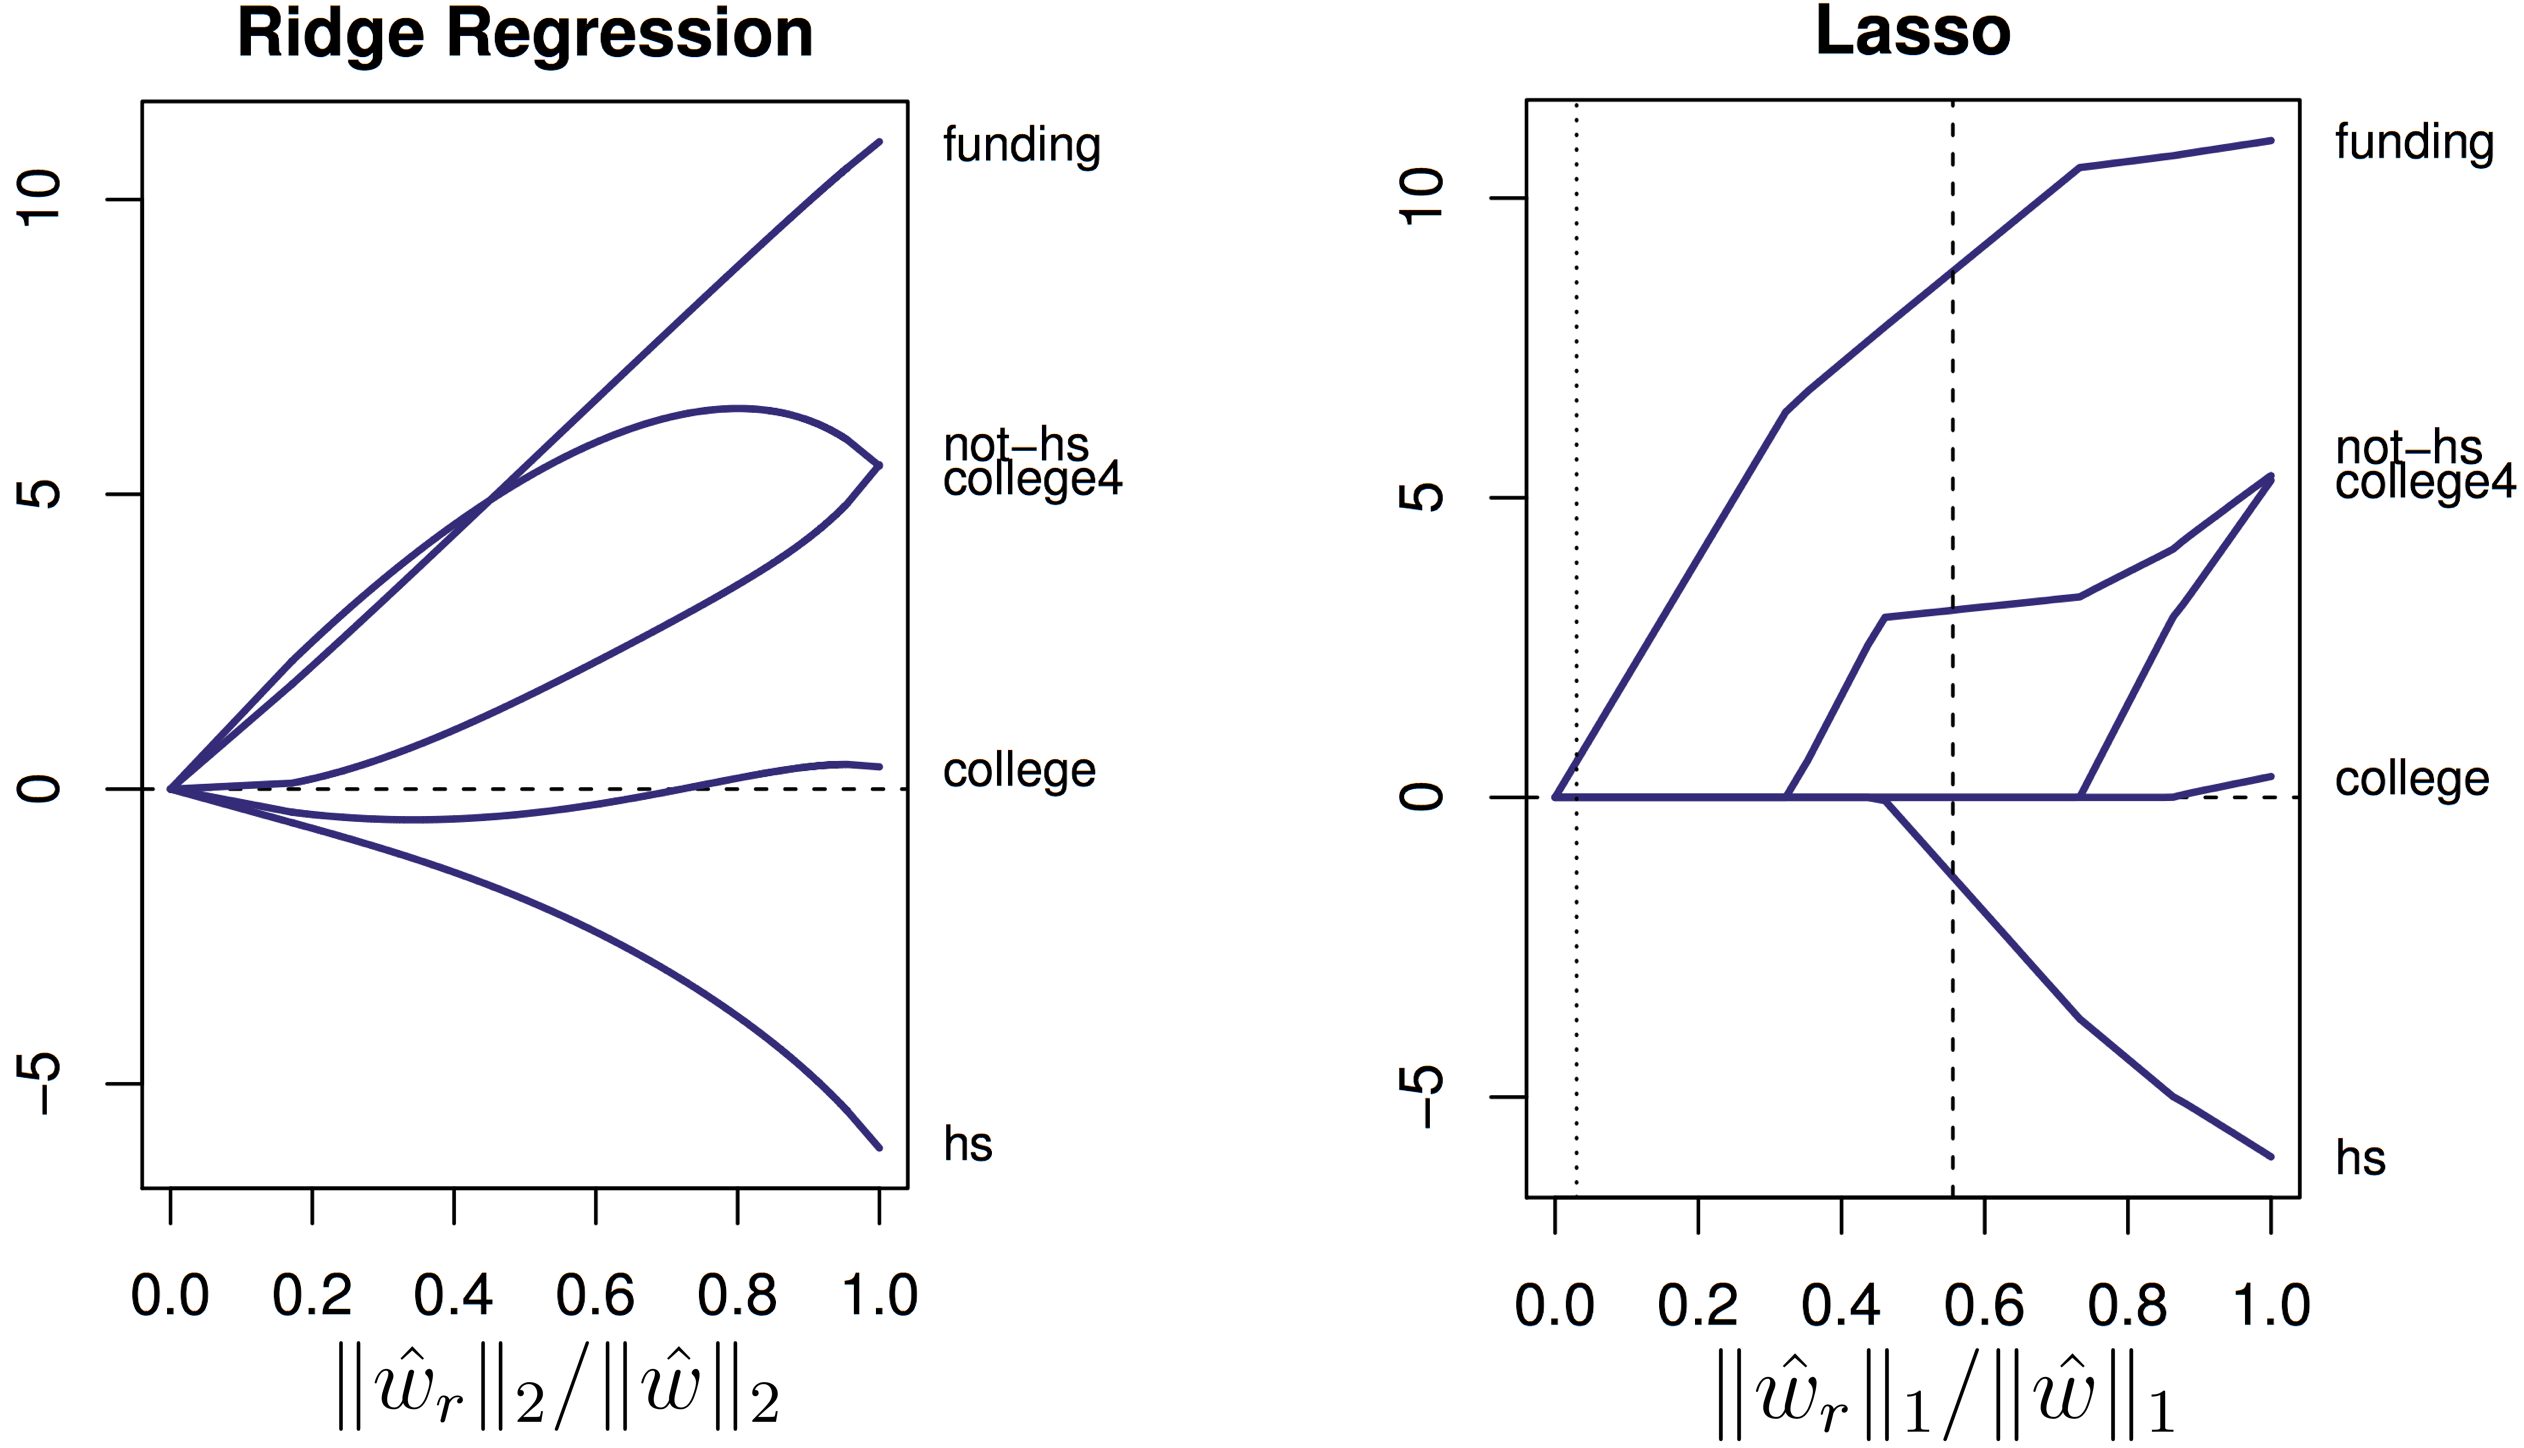
\includegraphics[height=0.7\textheight]{figures/lasso-ridge-paths-side-by-side}
\par\end{center}
\end{frame}

\begin{frame}{Lasso Gives Feature Sparsity: So What?}

Coefficient are $0$ $\implies$don't need those features. What's
the gain?

\begin{itemize}
\item Time/expense to compute/buy features

\item Memory to store features (e.g. real-time deployment)

\item Identifies the important features

\item Better prediction? sometimes

\item As a feature-selection step for training a slower non-linear model
\end{itemize}
\end{frame}

\section{Regularization and Sparsity}
\begin{frame}{Constrained Empirical Risk Minimization}
\begin{block}{Constrained ERM (Ivanov regularization)}
For complexity measure $\Omega:\cf\to[0,\infty)$ and fixed $r\ge0$,
\begin{align*}
\min_{f\in\cf}\; & \frac{1}{n}\sum_{i=1}^{n}\ell(f(x_{i}),y_{i})\\
\mbox{s.t.}\; & \Omega(f)\le r
\end{align*}
\end{block}

\begin{block}{Lasso Regression (Ivanov Form)}
The lasso regression solution for complexity parameter $r\ge0$ is
\[
\hat{w}=\argmin_{\|w\|_{1}\le r}\frac{1}{n}\sum_{i=1}^{n}\left\{ w^{T}x_{i}-y_{i}\right\} ^{2}.
\]
\end{block}
    $r$ has the same role as $\lambda$ in penalized ERM (Tikhonov).
\end{frame}

\begin{frame}{Ivanov vs Tikhonov Regularization }
\begin{itemize}
\item Let $L:\cf\to\reals$ be any performance measure of $f$
\begin{itemize}
\item e.g. $L(f)$ could be the empirical risk of $f$
\end{itemize}

\item For many $L$ and $\Omega$, Ivanov and Tikhonov are ``equivalent'':
\begin{itemize}
\item Any solution $f^{*}$ you could get from Ivanov, can also get from
Tikhonov.
\item Any solution $f^{*}$ you could get from Tikhonov, can also get from
Ivanov.
\end{itemize}
\item Can get conditions for equivalence from Lagrangian duality theory.
\item In practice, both approaches are effective.
\item We will use whichever that is more convenient. 
\end{itemize}
\end{frame}

\begin{frame}{Ivanov vs Tikhonov Regularization (Details) }
Ivanov and Tikhonov regularization are equivalent if:
\begin{enumerate}
\item For any choice of $r>0$, any Ivanov solution
\[
\minimizer{f_{r}}\in\argmin_{\substack{f\in\cf}
}L(f)\mbox{ s.t. }\Omega(f)\le r
\]
is also a Tikhonov solution for some $\lambda>0$. That is, $\exists\lambda>0$
such that
\[
\minimizer{f_{r}}\in\argmin_{f\in\cf}L(f)+\lambda\Omega(f).
\]


\item Conversely, for any choice of $\lambda>0$, any Tikhonov solution:
\[
\minimizer{f_{\lambda}}\in\argmin_{f\in\cf}L(f)+\lambda\Omega(f)
\]
is also an Ivanov solution for some $r>0$. That is, $\exists r>0$
such that
\[
\minimizer{f_{\lambda}}\in\argmin_{\substack{f\in\cf}
}L(f)\mbox{ s.t. }\Omega(f)\le r
\]
\end{enumerate}
\end{frame}

\begin{frame}{The $\ell_{1}$ and $\ell_{2}$ Norm Constraints}
\begin{itemize}
\item For visualization, restrict to 2-dimensional input space
\item $\cf=\left\{ f(x)=w_{1}x_{1}+w_{2}x_{2}\right\} $ (linear hypothesis
space)

\item Represent $\cf$ by $\left\{ \left(w_{1},w_{2}\right)\in\reals^{2}\right\} .$
\end{itemize}

\begin{columns}[t]

\column{.3\textwidth}
\begin{itemize}
\item $\ell_{2}$ contour: $w_{1}^{2}+w_{2}^{2}=r$
\end{itemize}
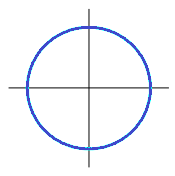
\includegraphics[height=0.25\textheight]{figures/l2Contour}


\column{.3\textwidth}
\begin{itemize}
\item $\ell_{1}$ contour: $\left|w_{1}\right|+\left|w_{2}\right|=r$ 
\end{itemize}
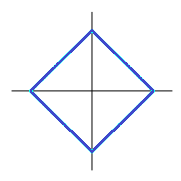
\includegraphics[height=0.25\textheight]{figures/l1Countour}
\end{columns}
Where are the ``sparse'' solutions?
\end{frame}

\begin{frame}{The Famous Picture for $\ell_{2}$ Regularization}

\begin{itemize}
\item $\minimizer{f_{r}}=\argmin_{w\in\reals^{2}}\sum_{i=1}^{n}\left(w^{T}x_{i}-y_{i}\right)^{2}\text{subject to }w_{1}^{2}+w_{2}^{2}\le r$
\end{itemize}
\begin{center}
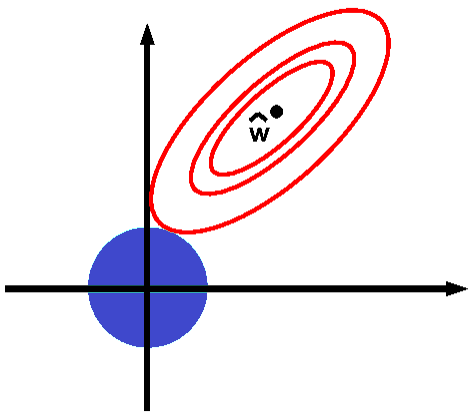
\includegraphics[height=0.5\textheight]{figures/l2LossConstraintPic}\vspace{-0.3cm}
\par\end{center}
\begin{itemize}
        \setlength\itemsep{1ex}
\item Blue region: Area satisfying complexity constraint: $w_{1}^{2}+w_{2}^{2}\le r$
\item Red lines: contours of $\hat{R}_{n}(w)=\sum_{i=1}^{n}\left(w^{T}x_{i}-y_{i}\right)^{2}$. 
\end{itemize}
\let\thefootnote\relax\footnotetext{\tiny{KPM Fig. 13.3}}
\end{frame}

\begin{frame}{The Famous Picture for $\ell_{1}$ Regularization}
\let\thefootnote\relax\footnotetext{\tiny{KPM Fig. 13.3}}
\begin{itemize}
\item $\minimizer{f_{r}}=\argmin_{w\in\reals^{2}}\frac{1}{n}\sum_{i=1}^{n}\left(w^{T}x_{i}-y_{i}\right)^{2}\text{subject to}\left|w_{1}\right|+\left|w_{2}\right|\le r$
\end{itemize}
\begin{center}
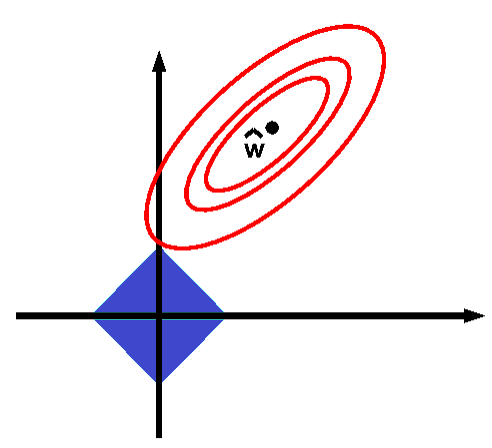
\includegraphics[height=0.5\textheight]{figures/l1LossConstraintPic}\vspace{-0.3cm}
\par\end{center}
\begin{itemize}
        \setlength\itemsep{1ex}
\item Blue region: Area satisfying complexity constraint: $\left|w_{1}\right|+\left|w_{2}\right|\le r$
\item Red lines: contours of $\hat{R}_{n}(w)=\sum_{i=1}^{n}\left(w^{T}x_{i}-y_{i}\right)^{2}$. 
\item $\ell_1$ solution tends to touch the \hl{corners}.
\end{itemize}
\end{frame}

\begin{frame}
    {Why does $\ell_1$ gives sparse solution?}
    \head{Geometric intuition}: Euclidean projection onto a convex set encourages solutions at corners or edges.
    \begin{itemize}
        \item $\hat{w}$ in red/green regions are closest to corners in the $\ell_1$ ball.
    \end{itemize}

\let\thefootnote\relax\footnotetext{\tiny{Fig from \href{https://arxiv.org/abs/1411.3230}{Mairal et al.'s Sparse Modeling for Image and Vision Processing} Fig 1.6}}
\begin{center}
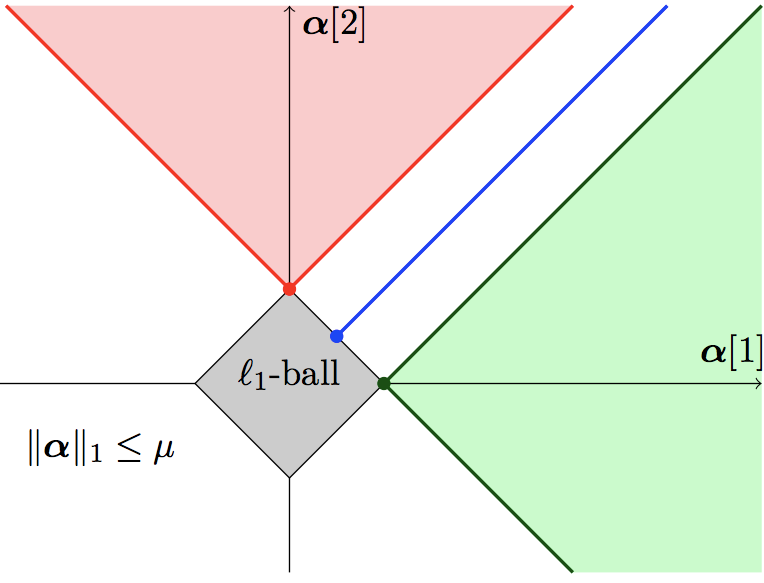
\includegraphics[height=0.5\textheight]{figures/projections-to-L1Ball}\vspace{-0.3cm}
\par\end{center}
\end{frame}

\begin{frame}
    {Why does $\ell_1$ gives sparse solution?}
    \head{Geometric intuition}: Euclidean projection onto a convex set encourages solutions at corners or edges.
    \begin{itemize}
        \item $\ell_2$ ball encourages solution in any direction equally. 
    \end{itemize}

\let\thefootnote\relax\footnotetext{\tiny{Fig from \href{https://arxiv.org/abs/1411.3230}{Mairal et al.'s Sparse Modeling for Image and Vision Processing} Fig 1.6}}
\begin{center}
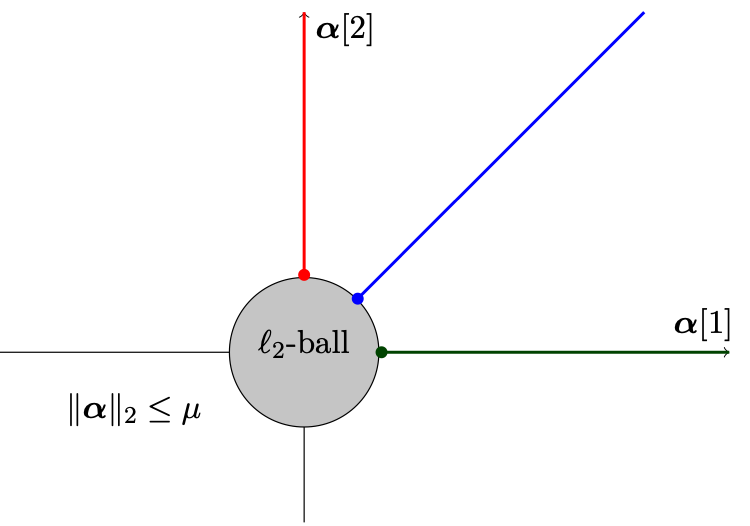
\includegraphics[height=0.5\textheight]{figures/projections-to-L2Ball}\vspace{-0.3cm}
\par\end{center}
\end{frame}

\begin{frame}
    {Why does $\ell_1$ gives sparse solution?}
    For $\ell_2$ regularization,
    \begin{itemize}
        \item As $w_i$ becomes smaller, there is less and less penalty 
            \begin{itemize}
                \item What is the $\ell_2$ penalty for $w_i=0.0001$?
            \end{itemize}
        \item The gradient goes to zero as $w_i$ moves towards zero 
    \end{itemize}

    For $\ell_1$ regularization,
    \begin{itemize}
        \item The function is \hl{non-smooth} and the gradient stays the same as the weights becomes smaller
        \item Thus it pushes them to exactly zero even if the weights are already tiny
    \end{itemize}

    (More discussion in lecture)
\end{frame}

\begin{frame}{The $\left(\ell_{q}\right)^{q}$ Constraint}
\begin{itemize}
\item Generalize to $\ell_{q}$ : $\left(\|w\|_{q}\right)^{q}=\left|w_{1}\right|^{q}+\left|w_{2}\right|^{q}$.
\item Contours of $\|w\|_{q}^{q}=\left|w_{1}\right|^{q}+\left|w_{2}\right|^{q}$:
\end{itemize}
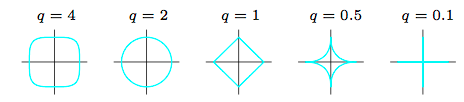
\includegraphics[width=0.8\columnwidth]{figures/LqNormContours}

\begin{itemize}
\item Note: $\|w\|_{q}$ is a norm if $q\ge1$, but not for $q\in\left(0,1\right)$
\item $\ell_q$ constraint when $q<1$ is non-convex, so hard to optimize
\item $\ell_0$ ($\|w\|_0$) is defined as the number of non-zero weights, i.e. subset selection
\end{itemize}
\end{frame}

\end{document}
